% $Id$

\section{Empirical study}
\label{sec:stat:impl}

In the field of \SPLs\ analysis, the use of probabilistic methods carries two practical applications.
The first one consists in calculating the probability of having a
feature in a specific product.
This allows us to efficiently assign resources by prioritizing those features with a high probability
of being included into the \SPL. The second application consists in estimating the testing coverage
in the product line, which allows us to calculate those products that can be generated in the testing process.

The idea to compute the probability of each feature is to hide all the
other features and then compute the resulting \SPL. This approach is
based on Proposition~\ref{prop:hid}. The problem with that Proposition
is that we cannot remove the features involved in restrictions
(requirement or exclusion) associated with the feature in which we are
interested. Hence, we need to add, to the non-hidden features, those that
appear in a restriction associated with the original one.
\begin{example}
  Let us assume that we want to compute the probability of $\fA$ in
  the term
  \begin{displaymath}
    \exclude{B}{C}{\require{C}{A}{P}}
    \end{displaymath}
    where \(P\) is a term without restrictions. Then we compute the
    probability of $\fA$ in the term
  \begin{displaymath}
    \exclude{B}{C}{\require{C}{A}{(Q\hide{\{\fA, \fB, \fC\}})}}
    \end{displaymath}

\end{example}

This section presents the results obtained from an experimental study to show the applicability and scalability of our
approach. In order to carry out this study, we have implemented a set of scripts to demonstrate
the applicability of the
probabilistic extension - of the denotational semantics - presented in this paper. The source code of the
scripts used in this section is available at the main project site
\footnote{\url{http://ccamacho.github.io/phd/resources/03_splap.tar}}. In essence, we perform two experiments.
The former focuses on measuring the performance of our proposed implementation for processing a feature model.
This means, given a feature model, calculating the time to
compute the probability of having each feature in the
valid products set.
The second experiment consists on analyzing the scalability of our proposed implementation.
The idea is to study if there is a correlation between the number of features of each type and the
processing time. The experiments have been executed in a computer with the following features: Intel(R)
Xeon(R) Quad-Core CPU E5-2670 @ 2.60GHz, 64 GB of RAM memory and Centos 7 Operating System.

The study described in this section seeks to answer the following questions:

\begin{itemize}
        \item \textbf{RQ1}: Is it possible to translate current graphical representations of feature models to
        support probabilistic information?
        \item \textbf{RQ2}: Is it possible to extend \fodaPA in such a way that
        translates the probabilistic information from the graphical representation to a formal representation?
        \item \textbf{RQ3}: What is the impact of applying probabilistic analysis methods to current feature models like \FODA?
\end{itemize}



%--------------------------------------------------------------------------------------------------------------------

\subsection{Model analysis}
\label{sec:stat:impl:model:analysis}

Firstly, we have carried out an experiment to
show the computing time required to calculate the probability of having
each feature in the set of valid products.
In order to run this experiment, a variability model consisting of
3000 features has been used.
This variability model
has been generated using BeTTy~\cite{sg12}, in specific
its web version\footnote{\url{https://betty.services.governify.io/}}.
Figure~\ref{fig:plot:betty:params} depicts the parameters used in the feature models
generator.

\begin{figure}[h]
        \centering
        \linefigure
        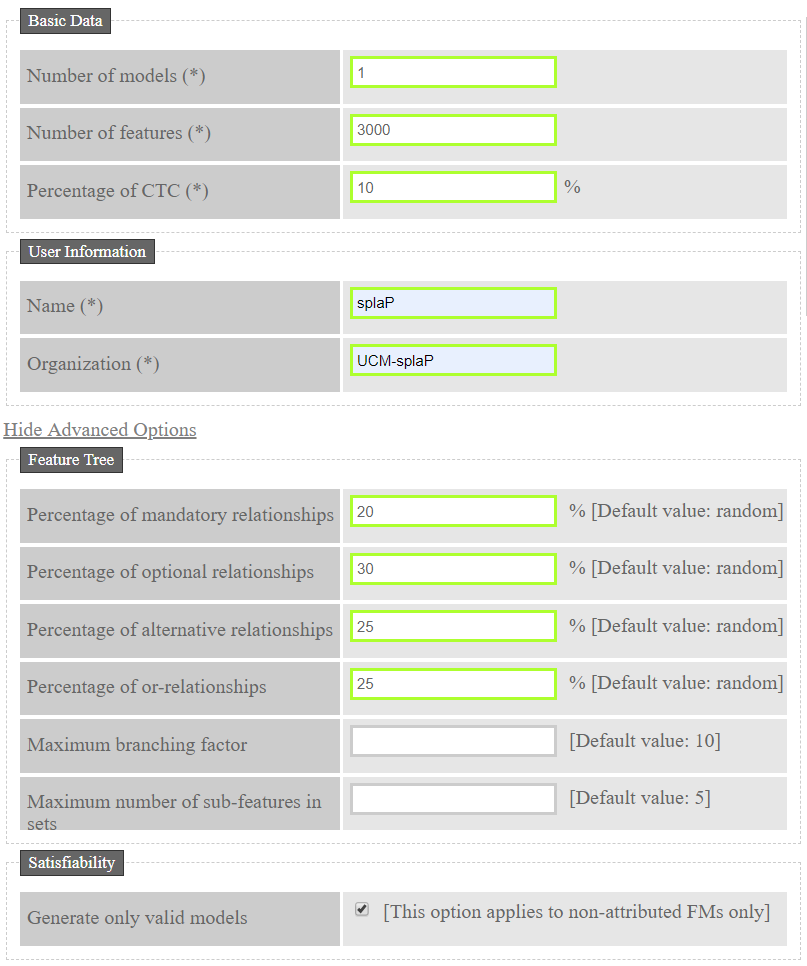
\includegraphics[width=0.8\hsize,angle=0]{BeTTy_website2.png}
        \linefigure
        \caption{BeTTy parameters.}\label{fig:plot:betty:params}
\end{figure}


BeTTy generates feature models based on a set of pre-defined parameters.
The meaning of these parameters focuses on how
BeTTy randomly generates these models.
In this case BeTTy requires 4 parameters, where the sum of the probabilities
for these parameters must be 1, that is:

\begin{itemize}
        \item The probability of having a mandatory feature.
        \item The probability of having an optional feature.
        \item The probability of having a feature in a \emph{choose-one} relationship.
        \item The probability of having a feature in a \emph{conjunction} relationship.
\end{itemize}

The values used for these parameters to generate the feature model are the following:

\begin{itemize}
        \item The probability of having a mandatory feature is 0.2.
        \item The probability of having an optional feature is 0.3.
        \item The probability of having a feature in a \emph{choose-one} relationship is 0.25.
        \item The probability of having a feature in a \emph{conjunction} relationship is 0.25.
\end{itemize}


The idea of using this configuration is to have the same probability for the different
relationships in the model, that is, we use a probability of 0.25 for both the
\emph{choose-one} and \emph{conjunction} relationships.
%We wanted to have the same probability of having the same relationships in the model, that is
%the reason of having 0.25 for the  \emph{choose-one} and \emph{conjunction} .
It is known that the optional features induce a  combinatorial explosion for creating
all the possible valid products from a feature model. Since we are interested on investigating
the performance of our approach, we use a probability of 0.3 for having optional features in
the model and a probability of 0.2 for having mandatory features.
The sum of all probabilities must be 1. If no weight is configured, all features and
relationships have a random weight, it being not possible to correlate the obtained results with
our model analysis.
Additionally, the percentage of cross-tree constraints is set to 10\%, which is not related to
the sum of the probabilities of the previous parameters.

\begin{figure}[h]
        \centering
        \linefigure
        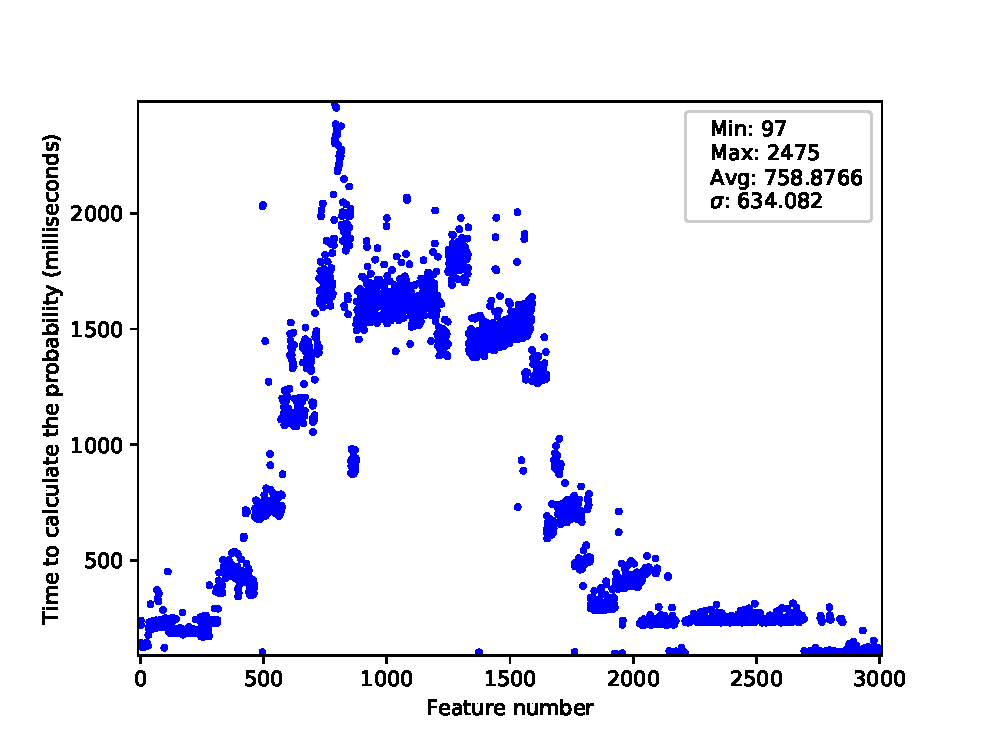
\includegraphics[width=0.8\hsize,angle=0]{plot_probs_times_FeatureModel3000.eps}
        \linefigure
        \caption{Computing time analysis for a model consisting of 3000 features.}\label{fig:plot:probs:times}
\end{figure}

Figure~\ref{fig:plot:probs:times} shows the obtained
results from this experiment, where the x-axis depicts
the ID of each generated feature and the y-axis represents
the time required to calculate the probability of having the feature in a final product.
%In this case, the total time to obtain the probability for all the features is linear with respect to the total length of the analyzed term
%\mncomment{Que quiere decir esto? Suena raro porque yo esperaria complejidad $O(2^n)$ siendo $n$ el numero de probabilidades que salen en el termino. Pero vamos, que yo no  se mucho de complejidad!}\ccomen{Es cierto, no lo demostramos ni lo analizamos}.
%\acomen{Yo simplemente quitaría esa frase, lo de que la complejidad es lineal}

% It is important to remark that there is a small variation in the processing time for
% calculating the probability of each single feature. We think that this variation is
% mainly caused by both the stochastic nature of the generated model and the
% inherent noise of the node where the experiment is launched (e.g. disk latencies, operating
% system overhead, memory paging, etc.) and, therefore, it is not related to the algorithm itself.

% Since the processing time for each feature is relatively low, it being around milliseconds, a single delay in
% the process scheduling may have a direct impact in the overall algorithm performance. Hence, this overhead
% can be considered insignificant since, in general, the time for processing each feature in the model ranges
% from 15 to 28 milliseconds.

From the graphic presented in Figure~\ref{fig:plot:probs:times} we can see that giving the fact that each feature is computed independently, the
computing time to calculate its probability depends on the feature position in the model.
Those features being lower in the model tree, will take more
time in being computed.

The model used in the experiments has been generated and processed 11 times, providing similar results
(see Table~\ref{execution_times}). That is, the
major part of the features require between 80 and 4599 milliseconds to be processed.
% , while there is a small
% portion of them requiring a processing time between 20 and 36 milliseconds. However, there are unusual situations
% where a feature require 60 milliseconds to be processed.

\begin{table}[h]
        \centering
        \begin{tabular}{|c|c|c|c|c|}
                \hline
                \textbf{Execution} & \textbf{Minimum} &  \textbf{Maximum} &  \textbf{Average} &  \textbf{Standard deviation} \\ \hline
                \textit{1}              & 97   & 2475  & 758.8766  & 634.082        \\ \hline
                \textit{2}              & 200  & 1950  & 612.8149  & 458.745        \\ \hline
                \textit{3}              & 80   & 3201  & 895.4566  & 701.569        \\ \hline
                \textit{4}              & 350  & 4054  & 975.4781  & 700.456        \\ \hline
                \textit{5}              & 89   & 2115  & 1002.5135 & 596.598        \\ \hline
                \textit{6}              & 236  & 1800  & 490.7506  & 399.927        \\ \hline
                \textit{7}              & 409  & 2900  & 684.1667  & 650.287        \\ \hline
                \textit{8}              & 360  & 3698  & 498.3847  & 710.136        \\ \hline
                \textit{9}              & 90   & 4599  & 642.8489  & 684.993        \\ \hline
                \textit{10}             & 150  & 2700  & 870.8184  & 688.013        \\ \hline
                \textit{11}             & 84   & 2379  & 769.187   & 623.544        \\ \hline
        \end{tabular}
        \caption{Computing time analysis table.}
        \label{execution_times}
\end{table}

\begin{figure}[h]
        \centering
        \begin{minipage}[b]{0.48\textwidth}
                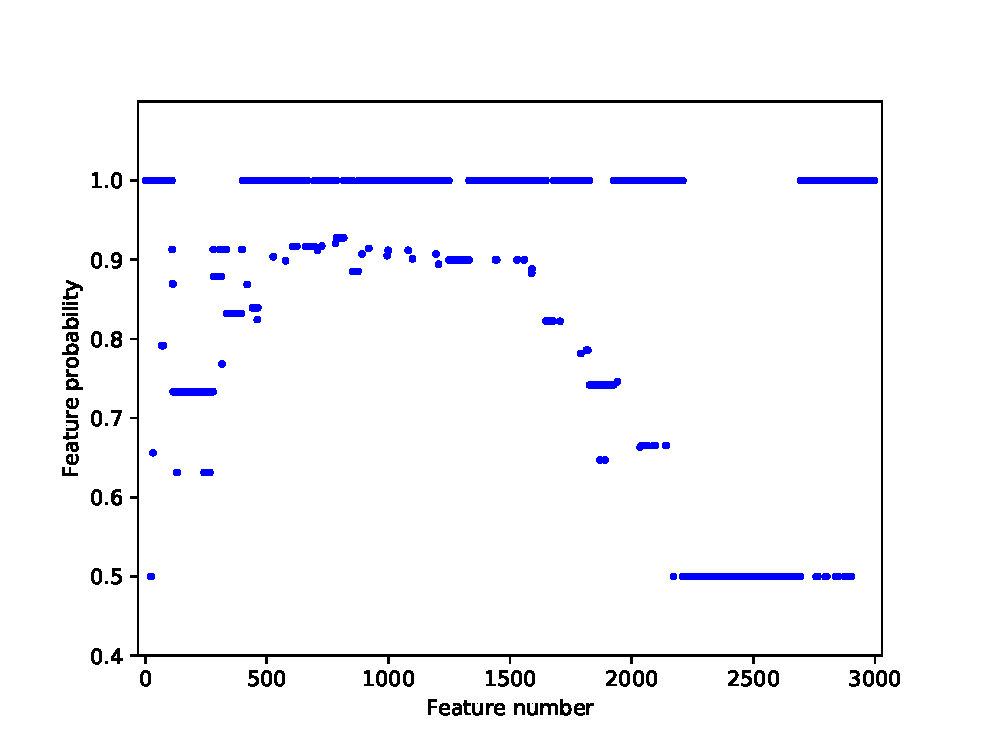
\includegraphics[width=\textwidth]{plot_probs_FeatureModel3000.eps}
\caption{Probabilistic analysis for a 3000 features model.}\label{fig:plot:probs:probs}
        \end{minipage}
        \hfill
        \begin{minipage}[b]{0.48\textwidth}
                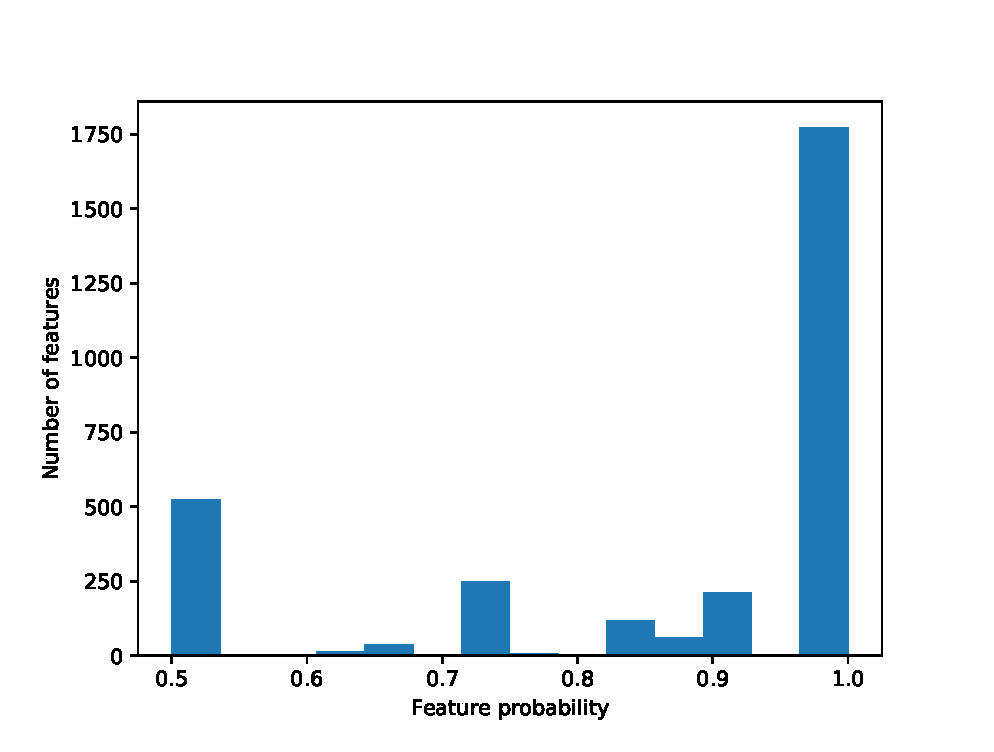
\includegraphics[width=\textwidth]{plot_probs_histogram_FeatureModel3000.eps}
        \caption{Probabilistic histogram for processing a 3000 features model.}\label{fig:plot:probs:probs:sorted}
        \end{minipage}
\end{figure}


Figure~\ref{fig:plot:probs:probs} shows the probability of each feature - in the analyzed model - to
be part of a final product, where the $x$-axis
represents the feature ID and the $y$-axis represents the probability.
Figure~\ref{fig:plot:probs:probs:sorted} represents a histogram of the calculated probabilities for a better
readability of the results. This chart clearly shows that there exist
different groups of features having a similar probability.
In this case, the probability of the major part
of the features ranges between 0.5 and 1.
%
Thus, there are 235 features with, at least, a probability equal to 0.90 of being in a final product.
As a conclusion, this analysis might allow us to establish that by testing only
the 7.83\% of the software product line components (235 features) we can ensure that,
will be tested components commonly distributed in the 90\% of the products generated using the referenced model.

It is important to differentiate the probabilities defined in BeTTy, which are used to generate a
feature model, and the probability - calculated from the model - to have a feature in a final
product.

For instance, if we configure BeTTy to generate a feature model using a probability
of 0.2 for having a mandatory feature, that means that 20\% of the generated features are mandatory.
However, that does not imply that these features be part of the 20\% of the generated products, because
the probability of having a feature in a final product depends on where this feature is placed in the
model. If a given mandatory feature is placed in a choose-one relationship, it is possible that
the other branch is used to generate the final product, discarding the mandatory feature.
Hence, we can not assume that these 20\% of the features will have a probability of 1 for being
installed in the products.

%For instance, if BeTTy is configured to generate mandatory features with a probability of 0.2 in a model, that will mean that those features will be presented in the model as mandatory with a probability of 0.2 and nothing else.
%The probability of those mandatory features in the model is not related directly with the probability of those features being part
%of let's say, the 20\% of the products, mostly, because it depends on the position of the features in the model for the
%products generation. In which case we can not assume that these 20\% of the features will have a probability of 1 for being installed
%in the products.


\subsection{Performance analysis}
\label{sec:stat:impl:performance:analysis}

Secondly, an evaluation to analyze the scalability of our approach
have been carried out. We are interested in investigating both the
execution time and the amount of memory required for processing a model
when the number of features increases.
Hence, we use different configurations for creating a wide
spectrum of variability models, which are randomly generated,
using a different number of features that ranges from 1.000 to 10.000 (in increments of one thousand per experiment).

Specifically for each case, that is, given a configuration and a number of features,
a model is randomly generated 30 times.
Additionally, for each model, 100 features are
randomly selected and, for each one, both the processing time and memory
required to calculate its probability are analyzed.



Table~\ref{scalaExperiment} shows the configurations used to generate the
variability models for this part of the empirical study,
where each configuration represents the set of probabilities chosen for each operator across the three experiments,
that is, \textit{Mandatory} represents the probability of having a mandatory feature,
 \textit{Optional} represents the probability of having an optional feature,
 \textit{Choose-one} represents the probability of having a feature in a \textit{choose-one} relation and
 \textit{Conjunction} represents the probability of having a feature in a \textit{conjunction} relation.

\begin{table}[h]
\centering
\begin{tabular}{|c|c|c|c|c|}
\hline
\textbf{Configuration} & \textbf{Mandatory} &  \textbf{Optional} &  \textbf{Choose-one} &  \textbf{Conjunction} \\ \hline
        \textit{1}              & 0.69  & 0.15  & 0.15  & 0.01  \\ \hline
        \textit{2}              & 0.5           & 0.15  & 0.15  & 0.2           \\ \hline
        \textit{3}              & 0.2           & 0.15  & 0.15  & 0.5   \\ \hline
\end{tabular}
\caption{Configuration of the scalability experiments.}
\label{scalaExperiment}
\end{table}

In this experiment, we have set the same values for the probabilities of the \textit{Optional}
and \textit{Choose-one} features. Hence, these will remain the same
across all the experiments and, thus, they should not interfere in the obtained results.
We start with a low probability of having a \textit{Conjunction} relationship in the model. In this
case, for the first experiment, we use a probability of 0.01, which is increased in the next configurations
to 0.2 and 0.5, respectively. This idea is to show the impact of the \textit{Conjunction} relationship in the time
and memory required for processing the models.

For each configuration, we have generated 30 models per number of features, that is, we generate
30 different models containing 1000 features, 30 different models containing 2000 features,
and so on until 10.000 features.

Figure~\ref{fig:plot:probs:boxplot_0_1} and figure~\ref{fig:plot:probs:boxplot_0_1_mem} show the execution time and the required amount of memory, respectively, for processing the variability models generated using \textit{Configuration 1}. In these models, only 1\% of the features have a conjunction relation. In general, the processing time when the number of features increases is linear. Only in few cases, where the number of features ranges from 5000 to 8000, the results provide anomalous values. This is mainly caused by the random nature of the generated models (30 for each case). On the contrary, the memory usage depicts that there are several groups where the memory usage remains constant, one group of models containing between 3,000 and 5,000 features and other group of models containing between 7,000 and 10,000 features. In summary, our implementation shows good scalability results for processing the models generated using \textit{Configuration 1}: it requires, in the worst case scenario, 215 ms and 0.32 GB of RAM to process the model.

\begin{figure}[h]
        \centering
        \begin{minipage}[b]{0.48\textwidth}
                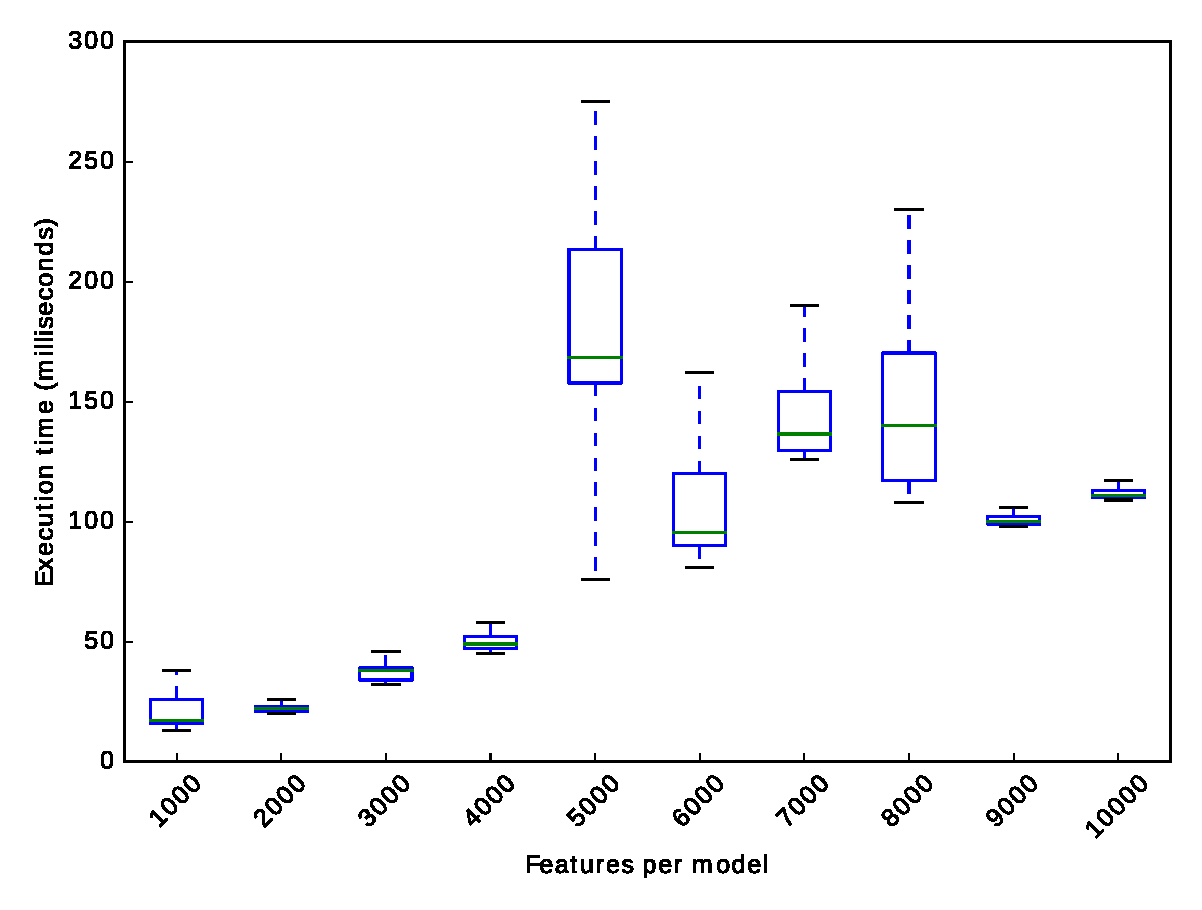
\includegraphics[width=\textwidth]{boxplot_0_1.eps}
                \caption{Execution time for processing models generated using \textit{Configuration 1}.}\label{fig:plot:probs:boxplot_0_1}
        \end{minipage}
        \hfill
        \begin{minipage}[b]{0.48\textwidth}
                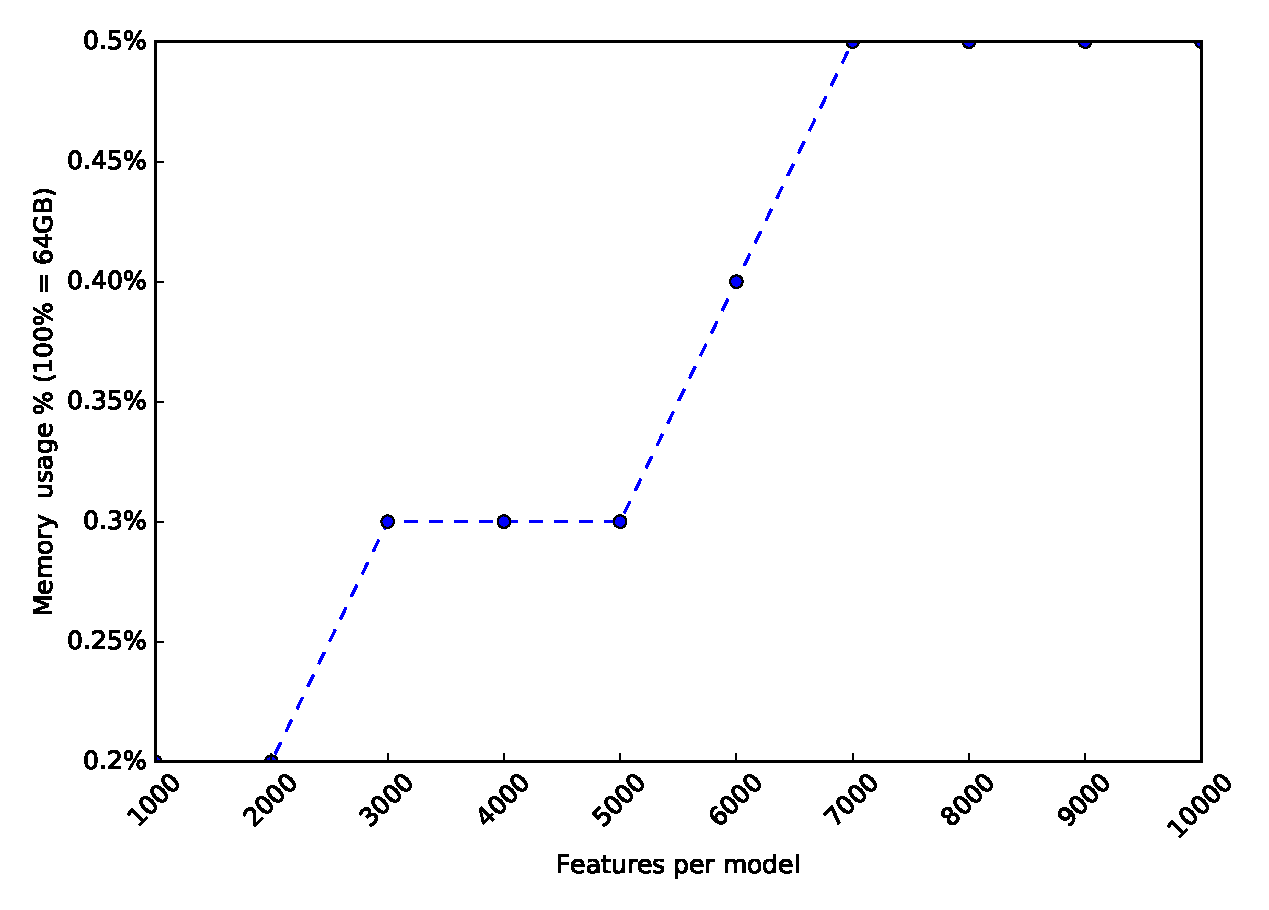
\includegraphics[width=\textwidth]{boxplot_0_1_mem.eps}
                \caption{Memory usage for processing models generated using \textit{Configuration 1}.}\label{fig:plot:probs:boxplot_0_1_mem}
        \end{minipage}
\end{figure}

Figure~\ref{fig:plot:probs:boxplot_0_2} and figure~\ref{fig:plot:probs:boxplot_0_2_mem} show the results for analyzing the models generated using \textit{Configuration 2}. It is important to remark that 20\% of the features in the generated models have a conjunction relation. In this case, both the execution time and memory usage for processing a model when the number of features increases are exponential. These charts clearly show a turning point when the model reaches 6,000 features and, therefore, the required processing time and  memory are significantly lower for those models that do not reach 6,000 features. However, the requirements to process the model in the worst case scenario, that is, using a model containing 10,000 features, are 300 sec. and 3.84 GB of RAM memory, which are acceptable.

\begin{figure}[h]
        \centering
        \begin{minipage}[b]{0.48\textwidth}
                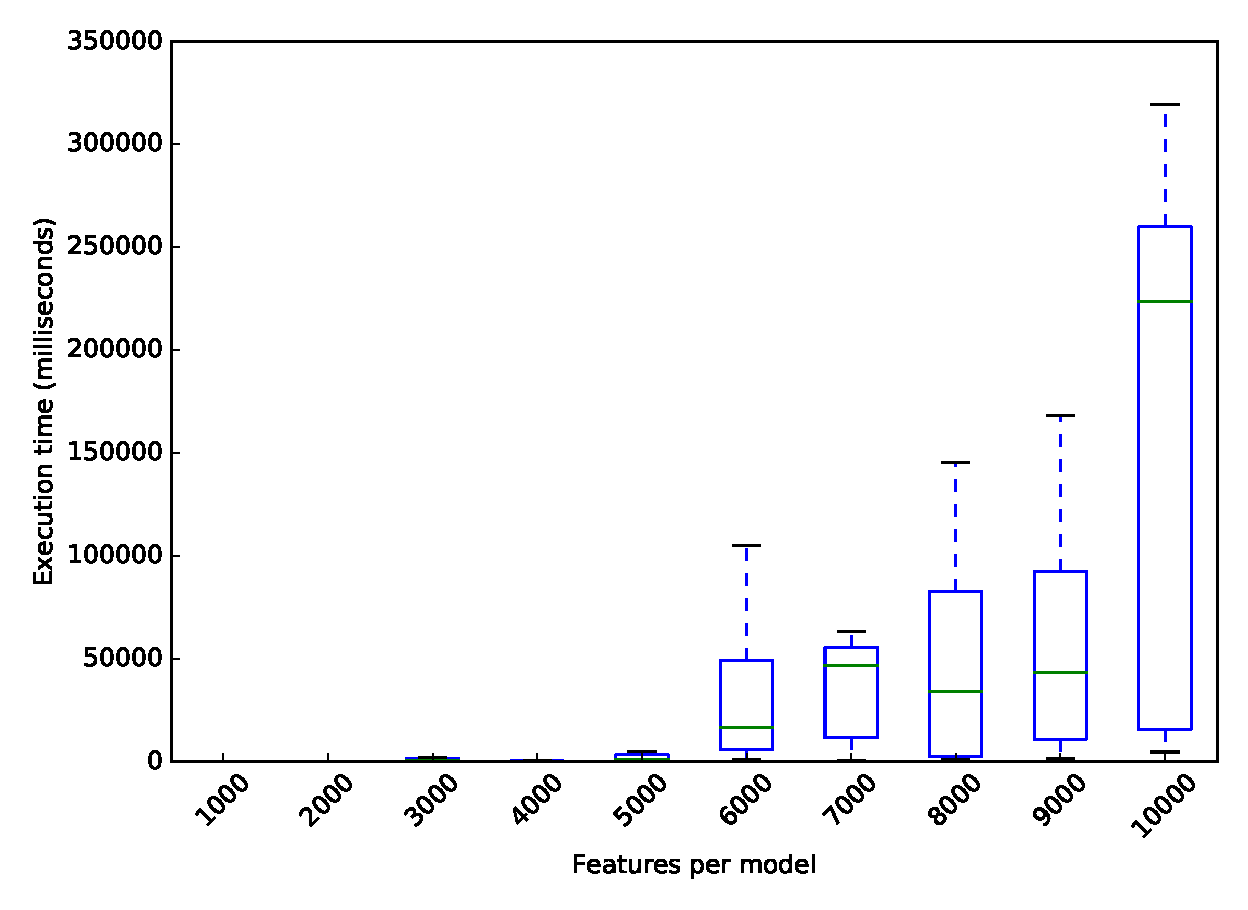
\includegraphics[width=\textwidth]{boxplot_0_2.eps}
                \caption{Execution time for processing models generated using \textit{Configuration 2}.}\label{fig:plot:probs:boxplot_0_2}
        \end{minipage}
        \hfill
        \begin{minipage}[b]{0.48\textwidth}
                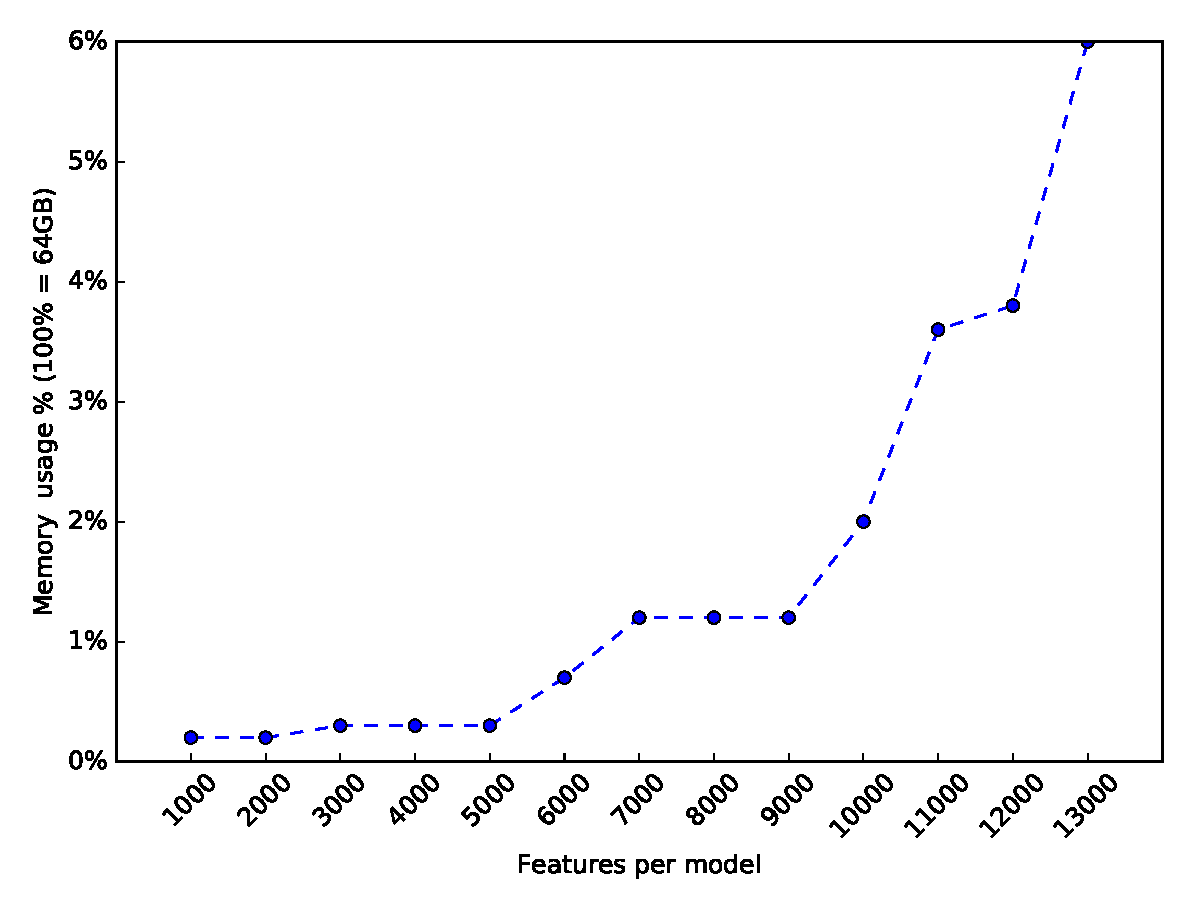
\includegraphics[width=\textwidth]{boxplot_mem.eps}
                \caption{Memory usage for processing models generated using \textit{Configuration 2}.}\label{fig:plot:probs:boxplot_0_2_mem}
        \end{minipage}
\end{figure}

Figure~\ref{fig:plot:probs:boxplot_0_5} and figure~\ref{fig:plot:probs:boxplot_0_5_mem} show the results for processing the models generated using \textit{Configuration 3}. In this case, half of the features in the model have a conjunction relation. Similarly to the previous experiment, these charts show that both the execution time and the memory usage for processing a model when the number of features increases are exponential. In the obtained results we can observe the same turning point detected in the previous models generated using  \textit{Configuration 2}, that is, when the model reaches 6,000 features. Model processing requirements, that is, execution time and memory usage, grow much faster for these models than for those based on previous configurations. Also, it is important to notice that the models containing 9,000 and 10,000 features cannot be processed due to memory limitations.

\begin{figure}[h]
        \centering
        \begin{minipage}[b]{0.48\textwidth}
                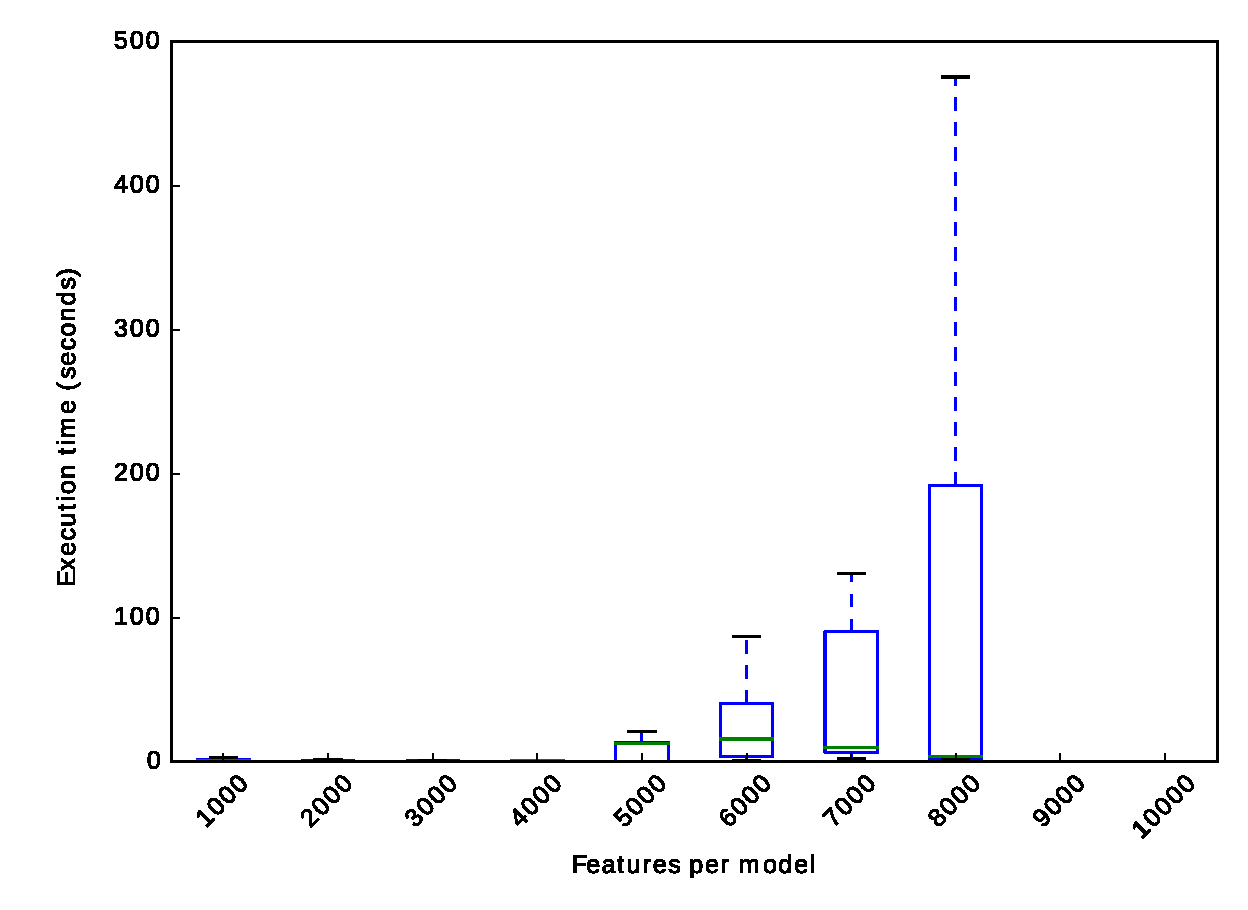
\includegraphics[width=\textwidth]{boxplot_0_5.eps}
                \caption{Execution time for processing models generated using \textit{configuration 3}.}\label{fig:plot:probs:boxplot_0_5}
        \end{minipage}
        \hfill
        \begin{minipage}[b]{0.48\textwidth}
                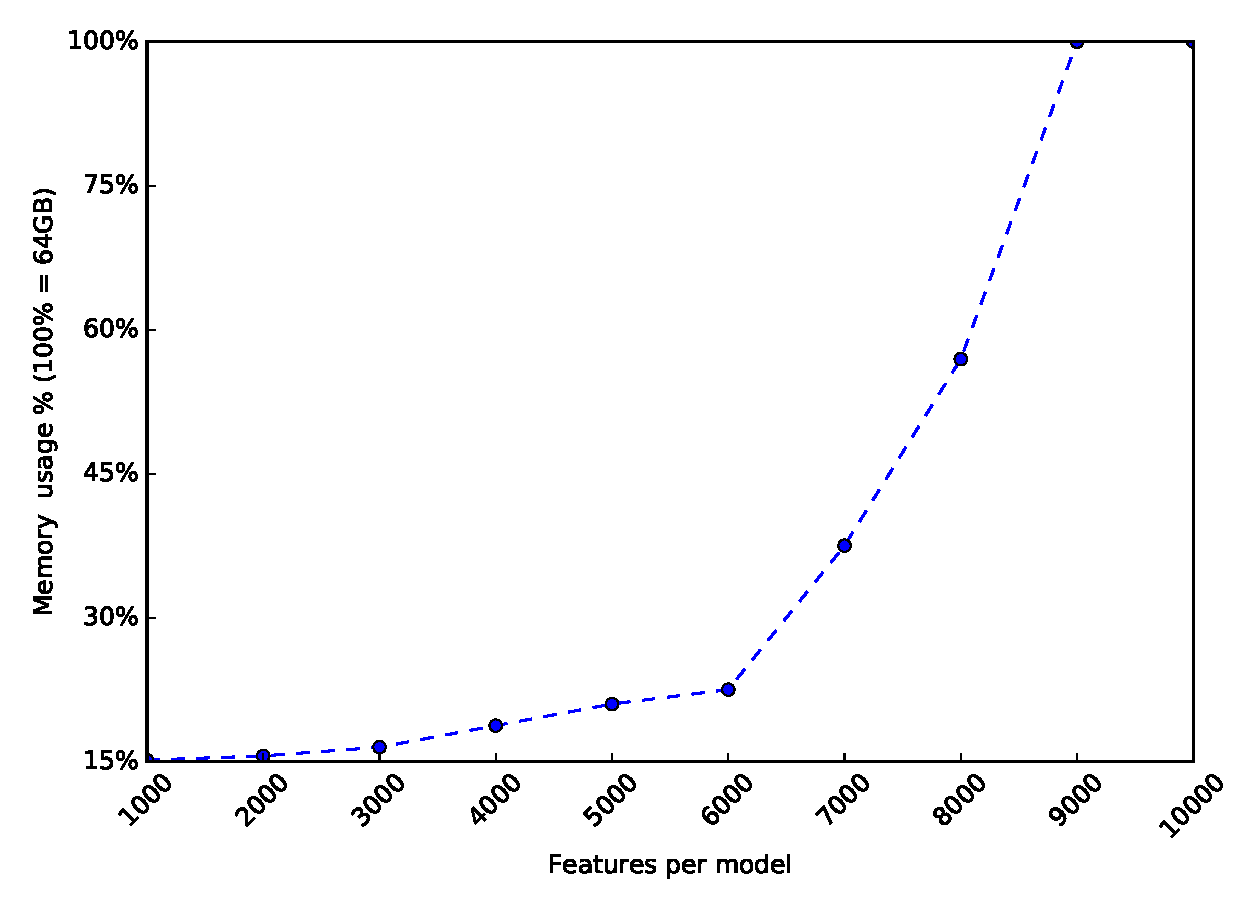
\includegraphics[width=\textwidth]{boxplot_0_5_mem.eps}
                \caption{Memory usage for processing models generated using \textit{configuration 3}.}\label{fig:plot:probs:boxplot_0_5_mem}
        \end{minipage}
\end{figure}


%%%------------------------------------------------------------------------------------------------------------------------------------------------

\subsection{Discussion of the results}
\label{sec:stat:impl:comp}

In this section we discuss the obtained results from the empirical study and
provide a comparison with the ones obtained using \fodaPA~\cite{acl13}
and the cost extension \fodaPAc~\cite{clc16}. Specifically, we are interested in
comparing the performance between the implementation of the probabilistic
extension and the implementation of the denotational semantic from
\fodaPA~\cite{acl13}. Also, we provide the answers for the research questions.

The experiments carried out in Section~\ref{sec:stat:impl:performance:analysis}
uses feature models containing a maximum of 10000 features. In general,
these results show that increasing the number of features having a conjunction relation
has a direct impact on the overall performance. In fact, increasing the number of features having
a conjunction relation generates a combinatorial explosion that hampers the processing of models.
First, the execution time to completely process a model significantly grows. Second, large amounts
of memory are required to store those combinations. In some cases, using large models with a high
percentage of features having a conjunction relation may cause a bottleneck in the memory system.
In fact, models generated using \textit{Configuration 3} with 9,000 and 10,000 features cannot be
processed using 64 GB of RAM. In this case,
the worst case scenario, which generates a model where the 50\% of the features are
placed in a conjunction relationship, requires approximately 500 seconds.

Figure~\ref{figure:tool:den:benchmark} shows the results of an experiment using
models containing different number of features, which ranges from $50$ to $300$.
In this case, we use the implementation of the denotational semantic from
\fodaPA~\cite{acl13} to process the models, which do not use probabilistic
information. If we use only the executions that successfully process the model,
the worst case scenario requires 786.126 seconds to process a model containing 150
features.

\begin{figure}[t]
        \centering
        \begin{minipage}{0.4\hsize}
        \begin{tabular}{|rrr|}
                        \hline
                Features&       Time (ms.)&    Products\\
                        \hline
                50 & 6 & 48 \\
                60 & 25 & 108 \\
                70 & 15 & 104 \\
                80 & 8 & 31 \\
                90 & 38 & 0 \\
                100 & 55 & 1404 \\
                110 & 13 & 12 \\
                120 & 2139 & 1 \\
                130 & 511 & 24802 \\
                140 & 7 & 6 \\
                150 & 786126 & 1312848 \\
                160 & 136 & 5670 \\
                170 & 42 & 398 \\
                \hline
        \end{tabular}
        \end{minipage}
        \begin{minipage}{0.4\hsize}
        \begin{tabular}{|rrr|}
                \hline
                Features&       Time (ms.)&    Products\\
                        \hline
180 & 744 & 6384 \\
190 & 1390 & 7232 \\
200 & 960000 & - \\
210 & 97770 & 800544 \\
220 & 263 & 51 \\
230 & 47 & 8 \\
240 & 65 & 29 \\
250 & 191 & 5920 \\
260 & 205 & 7296 \\
270 & 250 & 4301 \\
280 & 960000 & - \\
290 & 65 & 3 \\
300 & 960000 & - \\
                \hline
        \end{tabular}
        \end{minipage}
        \caption{Denotational benchmark from \cite{acl13}.\label{figure:tool:den:benchmark}}
\end{figure}




Also, based on the results published in \fodaPAc~\cite{clc16},
the models used for the simulations were processed in
an 8-node cluster. However, these models only contains 17 features.
Figure~\ref{fig:cluster} shows the algorithm behavior
which best time its approximately 300 seconds.

\begin{figure}[t]
        \centering
        \linefigure
        \resizebox{\columnwidth}{!}{%
                \begin{tabular}{|c|c|c|c|c|c|c|}
                        \cline{2-7}
                        \multicolumn{1}{c|}{} & 1 Worker & 2 Workers & 4 Workers & 8 Workers & 16 Workers & 32 Workers  \\
                        \hline
                        1 Node & 2010.44763303 & 1060.80047798 & 586.014445066 & 543.712262154 & 521.616870165 & 521.292215109 \\
                        \hline
                        2 Nodes & 2059.06947899 & 1046.87119007 & 575.115453959 & 296.285589933 & 366.384442091 & 341.007520199 \\
                        \hline
                        4 Nodes & 2031.25184584 & 1093.52087283 & 586.344302893 & 320.010899067 & 300.745616913 & 382.748430014 \\
                        \hline
                        8 Nodes & 2207.35427213 & 1143.951792 & 576.370896101 & 495.507214785 & 308.374300957 & 287.340030909 \\
                        \hline
                \end{tabular}
        }\\
        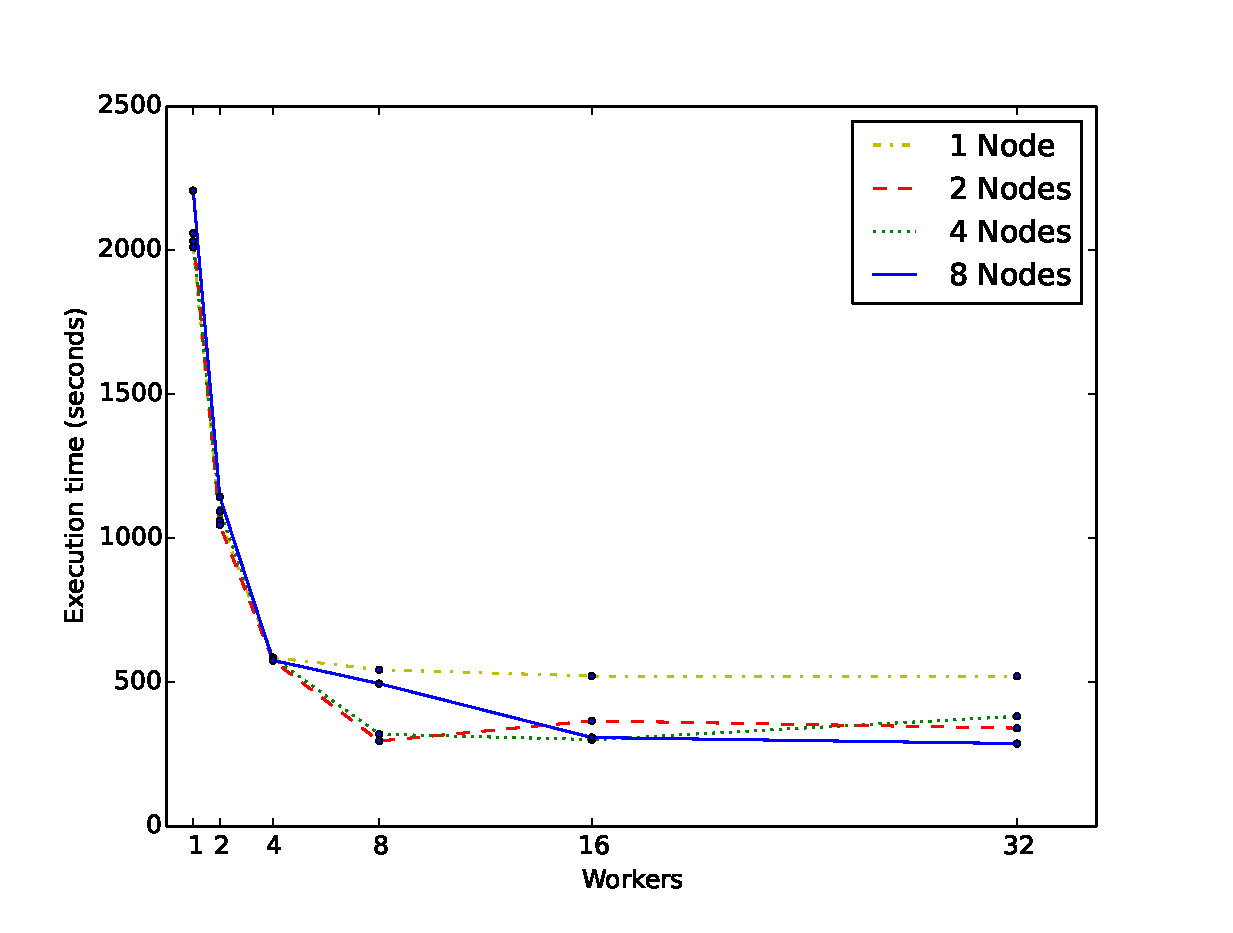
\includegraphics[width=0.7\hsize, height=5cm,angle=0]{plot_cluster.eps}
        \linefigure
        \caption{Cluster execution times for 1, 2, 4 and 8 nodes; and 1, 2, 4, 8, 16 and 32 workers  from~\cite{clc16}.}\label{fig:cluster}
\end{figure}

For those specific implementations and
simulations we can conclude
that the denotational semantics of the probabilistic
extension implementation improves dramatically
the performance
in comparison with the denotational semantics implementations
presented in previous works~\cite{acl13,clc16}.


Following, we provide the answers to the research questions.

\textbf{RQ1}: Is it possible to translate current graphical representations of feature models to
support probabilistic information?


In order to answer this question we have implemented the denotational semantic
of the probabilistic extension. Since our framework is based on \FODA, we
can state that the answer is yes, it is possible to translate current graphical
representations of feature models, like \FODA, to represent and support probabilistic
information.

\textbf{RQ2}: Is it possible to extend \fodaPA\ in such a way that
translates the probabilistic information from the graphical representation to a formal representation?

General use models have been proposed to model variability in software
product lines~\cite{tlll15, tllv15} and, specifically, for feature-oriented
systems~\cite{Dubslaff2015, Chrszon2018}.
Thus, all previous work focuses on
generic representations. However, this work is based on including probabilistic
information to the well-known feature model \FODA.
Based on our previous results~\cite{acl13,clc16}, together with the results
presented in this work, we can state that state it is possible to
describe a formal framework that translates the current graphical
definitions of feature models into to a probabilistic formal representation.

\textbf{RQ3}: What is the impact of applying probabilistic analysis methods
to current feature models like \FODA?

In order to answer this question we carried out some experiments using
our implementation of the denotational semantic \fodaPA~\cite{acl13}
and the cost extension \fodaPAc~\cite{clc16}. The results obtained
have been compared with the implementation of the probabilistic
extension. We observed that the latter is able to process larger
models faster, which provides a greater scalability when
the size of the model to be processed grows. Since the probabilistic extension
focuses on hiding  those features that do not affect the processing of the
probability of given feature for being part of a valid product, the required
tome for processing the model is considerably reduced.


%\begin{figure}[t]
%$$
%\begin{array}{ccc}
%\mathtt{Test}&\mathtt{Features}& \mathtt{Time}\\
%\#1& \feature{A},\feature{B} & 10\ units\\
%\#2& \feature{C},\feature{D} & 15\ units\\
%\#3& \feature{A},\feature{C},\feature{D} & 8\ units\\
%\#4& \feature{C},\feature{B} & 9\ units\\
%\end{array}
%$$
%\caption{Input parameter: test suite\label{fig:input:parameter}}
%\end{figure}

%We have two open issues:
%\begin{description}
%\item[Unit testing]  Let $P$ be a software product line, and $T_{unit}$ be a
%  test suite. Each test checks the correctness of a feature (i.e, %\feature{A} or \feature{B}).
%  We can compute the \emph{probability} of a feature. We test before those features with bigger probability.
%  \begin{itemize}
%  \item We can calculate the most frequent set of features in $P$ to test.
  %\item  We can provide a coverage of the test suite taking into account the percentage of appearance of each feature.
  %\end{itemize}

%\item[Integration testing] We have a test suite $T_{integration}$ where each test checks
%  the integration of a product.
%  Let us note that the integration of the product $\{\feature{A},\feature{B}\}$  can be different than
%  the integration of $\{\feature{A}, \feature{B},\feature{C}\}$.
%  \begin{itemize}
%  \item Which tests of the suite can be applied in this SPL?
 % \item What is the coverage of each test suite?
 % \end{itemize}


%\end{description}


%Next step is to associate to each integration test the time that
%it needs to be completed.
%For instance in Figure~\ref{fig:input:parameter} we represent some integration tests and the
%time that they need to be completed.



%\begin{quote}
%\emph{Let us consider an integration test suite and a probabilistic SPL $P$.
%If we only have $n$ time units, which is the \emph{best set} of tests
%to check the correctness of $P$? We say that a test is better than another
%test if its representativity (the probability to perform these features together) is higher.}
%\end{quote}

%\bprop
%        The previous problem is NP-hard\ccomen{I propose the transformation into the Subset Sum problem.}.
%\eprop

%Next we define the subset sum problem.

%\bdfn
%    Let $A = \{a_1, a_2, \ldots, a_n\}$ be a  set of natural numbers and $s$ be  a positive integer.
%    The subset sum problem checks if there is a subset $A'\subseteq A$ such that:  $$\sum_{a\in A'} = s$$
%\edfn

%In our previous problem we have a set of pairs $B=\{(p_{1},t_{1}),(p_{2},t_{2}),\ldots,(p_{n},t_{n})\}$ where
%$p_{i}$ is the probability to perform the test $i$ and $t_{i}$ is the time needed to perform this test, and
%two constants $P$ and $T$. $P$ will represent a probability value and $T$ a time value.
%We are looking for those pairs $(p_{i},t_{i}),\ldots,(p_{j},t_{j})\in B$ that
%$$
%\begin{array}{ll}
%p_{i}+\ldots +p_{j} &\geq P\\
%t_{i}+\ldots +t_{j} &\leq T\\
%\end{array}
%$$

%Let us consider that $p_{i}=t_{i}={a_i}$ and $P=T=s$.
%We can rewrite the previous problem into

%$$
%\left.
%\begin{array}{ll}
%a_{i}+\ldots +a_{j} &\geq s\\
%a_{i}+\ldots +a_{j} &\leq s\\
%\end{array}
%\right\}=
%a_{i}+\ldots +a_{j} = s\
%$$

%And we have the subset sum problem\ccomen{Please check because $p_{i}$ and $t_{i}$ can be reals while $s_{i}$ are integers}.


%\begin{enumerate}
%        \item We can create a GA to solve this problem.
%        \item We have that this problem is FPTAS~\cite{Ibarra:1975:FAA:321906.321909}.
%\end{enumerate}



%In order to obtain a set of tests that holds the previous issues, we propose
%two implementations.
%The first one is using a dynamic algorithm while the second one to use a genetic algorithm.

%\subsection{Dynamic algorithm}

% We adapted the dynamic algorithm of 0-1 Knapsack problem
%to our problem and we implemented it in python.


%We define a matrix $A$, where $A(i,j)$ contains the
%maximum value that can be attained from considering
%only the sum of the first i tests' probability that need at most j time units.


%$$
%A(i,j)=
%\left\{
%        \begin{array}{lll}
%        0 &\hspace*{3em}&\si i=0 \lor j = 0\\
%        A(i-1,j) & & \si t_i>j\\
%        \max{(A(i-1,j),p_{i}+A(i-1,j-t_i))} &&\si t_i \leq j
%        \end{array}
%\right.
%$$

%In our case, we will say that $A(n,T)$ is the solution if the sum of the  percentages
%of all elements involved in this solution is bigger than or equal to $P$. Otherwise we do not have a solution.


%For instance, in Table~\ref{figure:input:parameters} there are presented a set of 24
%different tests with their time consuming and its probability.
%For instance the first element, t1,9,150, means the test t1 needs 9 time units to be completed
%and the value associated with this test is 150\footnote{We could put here a measure, the probability or anything}.

%\begin{table}
%\centering

%\selectfont
%{\tt
%\begin{tabular}{|l|l|l|}
%\hline
%\#1,9,150 &
%\#2,13,35&
%\#3,153,200\\
%\#4,50,160&
%\#5,15,60&
%\#6,68,45\\
%\#7,27,60&
%\#8,39,40&
%\#9,23,30\\
%\#10,52,10&
%\#11,11,70&
%\#12,32,30\\
%\#13,24,15&
%\#14,48,10&
%\#15,73,40\\
%\#16,42,70&
%\#17,43,75&
%\#18,22,80\\
%\#19,7,20&
%\#20,18,12&
%\#21,4,50\\
%\#22,30,10&
%\#23,90,1&
%\#24,200,150\\
%\hline
%\end{tabular}}
%\caption{Input parameter (test,time,value) for the test selection algorithm.\label{figure:input:parameters}}
%\end{table}

% \begin{figure}[t]
% \centering
% includegraphics[scale=1]{GA_Flowchart_4}
% \caption{Scheme of GA.\label{scheme:genetic:algorithm}}
% \end{figure}





% After executing the dynamic algorithm, with the following input parameters a)
% the data presented in Table~\ref{figure:input:parameters} and T (the maximum time value) equals to 500,
% we obtain that {\tt \#1, \#2, \#3, \#4, \#5,
% \#7, \#8, \#9, \#11, \#12, \#16, \#17,
% \#18, \#19} and {\tt \#21}       conforms the final solution, and P =  1130.


% \subsection{Genetic Algorithm}

% Next we perform a genetic algorithm to discover a better solution.
% The GA structure is in Figure~\ref{scheme:genetic:algorithm}.
% With this algorithm we obtain values bigger than 1130.






% \subsubsection{Representation}
% We represent the possible solutions (those tests that hold the conditions) as follows:
% \begin{itemize}
%         \item Genotype: Given $n$ tests, we represent a solution with a binary (1/0) string
% of length $n$ where the position i determines whether the ith-test is included or not.
% The genotype space is complete, that is, any valid solution can be mapped in this array.
%         \item Phenotype: There are only some genotypes that are \emph{correct}. These are
% those that taking the $n'$, with $n'\leq n$ first $1$ bits from left to right of a genotype, we have that the sum of
% the time values associated with these tests is lower than or equal to T,
% and that the representativity of these tests is $\geq P$.
% \end{itemize}


% \subsubsection{Initial Population}
% We execute the algorithm with the parameters presented in Figure~\ref{fig:parameters:initial:population} in order to show
% how many initial population do we need.
% There is an interesting effect that this experiment reveals.
% The first and second graphs indicate that for populations smaller than 50 the chance for premature convergence seems to be rather high.
% Therefore we will consider that a good candidate for initial population is 500.

% \begin{figure}[t]
% \centering

% \begin{minipage}{0.45\hsize}\centering
%         \textbf{x}=10

% \includegraphics[scale=0.3]{graphs_basea/basea_diff_raw}
% \end{minipage}
% \begin{minipage}{0.4\hsize}\centering

%         \textbf{x}=50
% \includegraphics[scale=0.3]{graphs_baseb/baseb_diff_raw}

% \end{minipage}


% \begin{minipage}{0.45\hsize}\centering
%         \textbf{x}=200

% \includegraphics[scale=0.3]{graphs_based/based_diff_raw}
% \end{minipage}
% \begin{minipage}{0.4\hsize}\centering

%         \textbf{x}=500
% \includegraphics[scale=0.3]{graphs_basec/basec_diff_raw}

% \end{minipage}

% {\centering
% %\fontsize{7}{9}
% %\selectfont

% \begin{tabular}{|l|l|}
% \hline
% Representation  &Binary strings of length n\\
% Recombination   &One point crossover\\
% Recombination probability &     80\\
% Mutation        & Swap Mutator \\
% Mutation probability    & 2\% \\
% Parent selection        & Roulette\\
% Survivor selection      & Generational\\
% Population size         & \textbf{x} \\
% Termination condition   & Terminate the evolution based on the fitness stats\\
% Generations     & 100 \\
% \hline
% \end{tabular}}

% \caption{Comparing initial population\label{fig:parameters:initial:population}.}
% \end{figure}



% \subsubsection{Recombination probability}
% Next we study the effect of changing the recombination probability.
% In Figure~\ref{fig:parameters:recombination} we show the max fitness, average fitness and
% minimum fitness of the population, in each generation, using the probability values 0.1, 0.4, 0.8 and 1 for recombination.
% We will use 0.8 in the rest of experiments because a) we obtain the maximum fitness, and b) the difference between maximum and minimum is low.

% Let us also note that adding more values of recombination probability (i.e, 100\%), that is also presented in
%  Figure~\ref{fig:parameters:recombination} does not imply to have better fitness solutions. So, this value should be high
% but not 100\%.

% \begin{figure}[t]

% \centering

% \begin{minipage}{0.5\hsize}\centering
%         \textbf{x}=0.1

% \includegraphics[scale=0.3]{graphs_basee/basee_maxmin_fitness}
% \end{minipage}
% \begin{minipage}{0.4\hsize}\centering

%         \textbf{x}=0.4
% \includegraphics[scale=0.3]{graphs_basef/basef_maxmin_fitness}

% \end{minipage}


% \begin{minipage}{0.50\hsize}\centering
%         \textbf{x}=0.8

% \includegraphics[scale=0.3]{graphs_baseg/baseg_maxmin_fitness}
% \end{minipage}
% \begin{minipage}{0.4\hsize}\centering

%         \textbf{x}=1
% \includegraphics[scale=0.3]{graphs_baseh/baseh_maxmin_fitness}

% \end{minipage}


% {\centering
% %\fontsize{7}{9}
% %\selectfont

% \begin{tabular}{|l|l|}
% \hline
% Representation  &Binary strings of length n\\
% Recombination   &One point crossover\\
% Recombination probability &     \textbf{x}\\
% Mutation        & Swap Mutator \\
% Mutation probability    & 2\% \\
% Parent selection        & Roulette\\
% Survivor selection      & Generational\\
% Population size         & 500 \\
% Termination condition   & Terminate the evolution based on the fitness stats\\
% Generations     & 100 \\
% \hline
% \end{tabular}}

% \caption{Comparing recombination probability\label{fig:parameters:recombination}.}
% \end{figure}

% \subsubsection{Mutation operator}

% We define two mutation operators in the chromosomes. The first one: swap means to change
% the element i with the element j. The second one: Integer range, means that we change a bit
% randomly.

% In our algorithm we are able to use both mutators operators.
% In Figure~\ref{fig:parameters:mutation:operator} the effects of executing swap, integer range or both
% are presented.

% We can observe that only swap let the fitness score to be regular with respect to the number of generations.
% When we change randomly a bit in the chromosomes then the fitness score cannot be predictable.

% \begin{figure}[t]

% \centering

% \begin{minipage}{0.5\hsize}\centering
%         \textbf{x}=Swap

% \includegraphics[scale=0.3]{graphs_basei/basei_maxmin_fitness}
% \end{minipage}
% \begin{minipage}{0.45\hsize}\centering

%         \textbf{x}=Swap and Integer Range

% \includegraphics[scale=0.3]{graphs_basej/basej_maxmin_fitness}

% \end{minipage}

% \begin{minipage}{0.5\hsize}\centering
%         \textbf{x}=Integer Range

% \includegraphics[scale=0.3]{graphs_basek/basek_maxmin_fitness}
% \end{minipage}
% %\begin{minipage}{0.45\hsize}\centering

% {\centering

% %\fontsize{7}{9}
% %\selectfont
% \begin{tabular}{|l|l|}
% \hline
% Representation  &Binary strings of length n\\
% Recombination   &One point crossover\\
% Recombination probability &     0.8\\
% Mutation        & \textbf{x} \\
% Mutation probability    & 2\% \\
% Parent selection        & Roulette\\
% Survivor selection      & Generational\\
% Population size         & 500 \\
% Termination condition   & Terminate the evolution based on the fitness stats\\
% Generations     & 100 \\
% \hline
% \end{tabular}}
% %\end{minipage}

% \caption{Comparing Mutation Operators\label{fig:parameters:mutation:operator}.}
% \end{figure}

% \subsubsection{Parent Selection}

% Finally we compare the parent selection methodology used in our algorithm.
% We implement three kind of selections: Rank, Roulette and Tournament.
% In our experiments we decided to use Roulette because it is always increasing,
% and it seems that we can continue improving the valuation of the set of tests over time.
% Moreover the others seem to be saturated.
% \begin{figure}[t]

% \centering

% \begin{minipage}{0.5\hsize}\centering
%         \textbf{x}=Rank

% \includegraphics[scale=0.3]{graphs_baser/baser_maxmin_fitness}
% \end{minipage}
% \begin{minipage}{0.4\hsize}\centering

%         \textbf{x}=Roulette
% \includegraphics[scale=0.3]{graphs_bases/bases_maxmin_fitness}

% \end{minipage}

% \begin{minipage}{0.50\hsize}\centering
%         \textbf{x}=Tournament

% \includegraphics[scale=0.3]{graphs_baset/baset_maxmin_fitness}
% \end{minipage}

% %\begin{minipage}{0.45\hsize}\centering


% {\centering
% %\fontsize{7}{9}
% %\selectfont
% \begin{tabular}{|l|l|}
% \hline
% Representation  &Binary strings of length n\\
% Recombination   &One point crossover\\
% Recombination probability &     0.8\\
% Mutation        & Swap \\
% Mutation probability    & 2\% \\
% Parent selection        & \textbf{x}\\
% Survivor selection      & Generational\\
% Population size         & 500 \\
% Termination condition   & Terminate the evolution based on the fitness stats\\
% Generations     & 100 \\
% \hline
% \end{tabular}}
% %\end{minipage}

% \caption{Comparing parent selection\label{fig:parameters:parent:selection}.}
% \end{figure}

%%% Local Variables:
%%% mode: latex
%%% TeX-master: "main"
%%% End:
